%% LyX 2.3.5.2 created this file.  For more info, see http://www.lyx.org/.
%% Do not edit unless you really know what you are doing.
\documentclass[english]{article}
\usepackage[T1]{fontenc}
\usepackage[latin9]{inputenc}
\usepackage{graphicx}

\makeatletter
\@ifundefined{date}{}{\date{}}
\makeatother

\usepackage{babel}
\begin{document}
\title{\underline{Pr�ctica 1: Introducci�n a R}}
\author{\underline{Alumno:}Pablo Alonso}

\maketitle
Para correr el script: 

- \$chmod +x script.R 

- \$./script.R

\subsection*{2)}

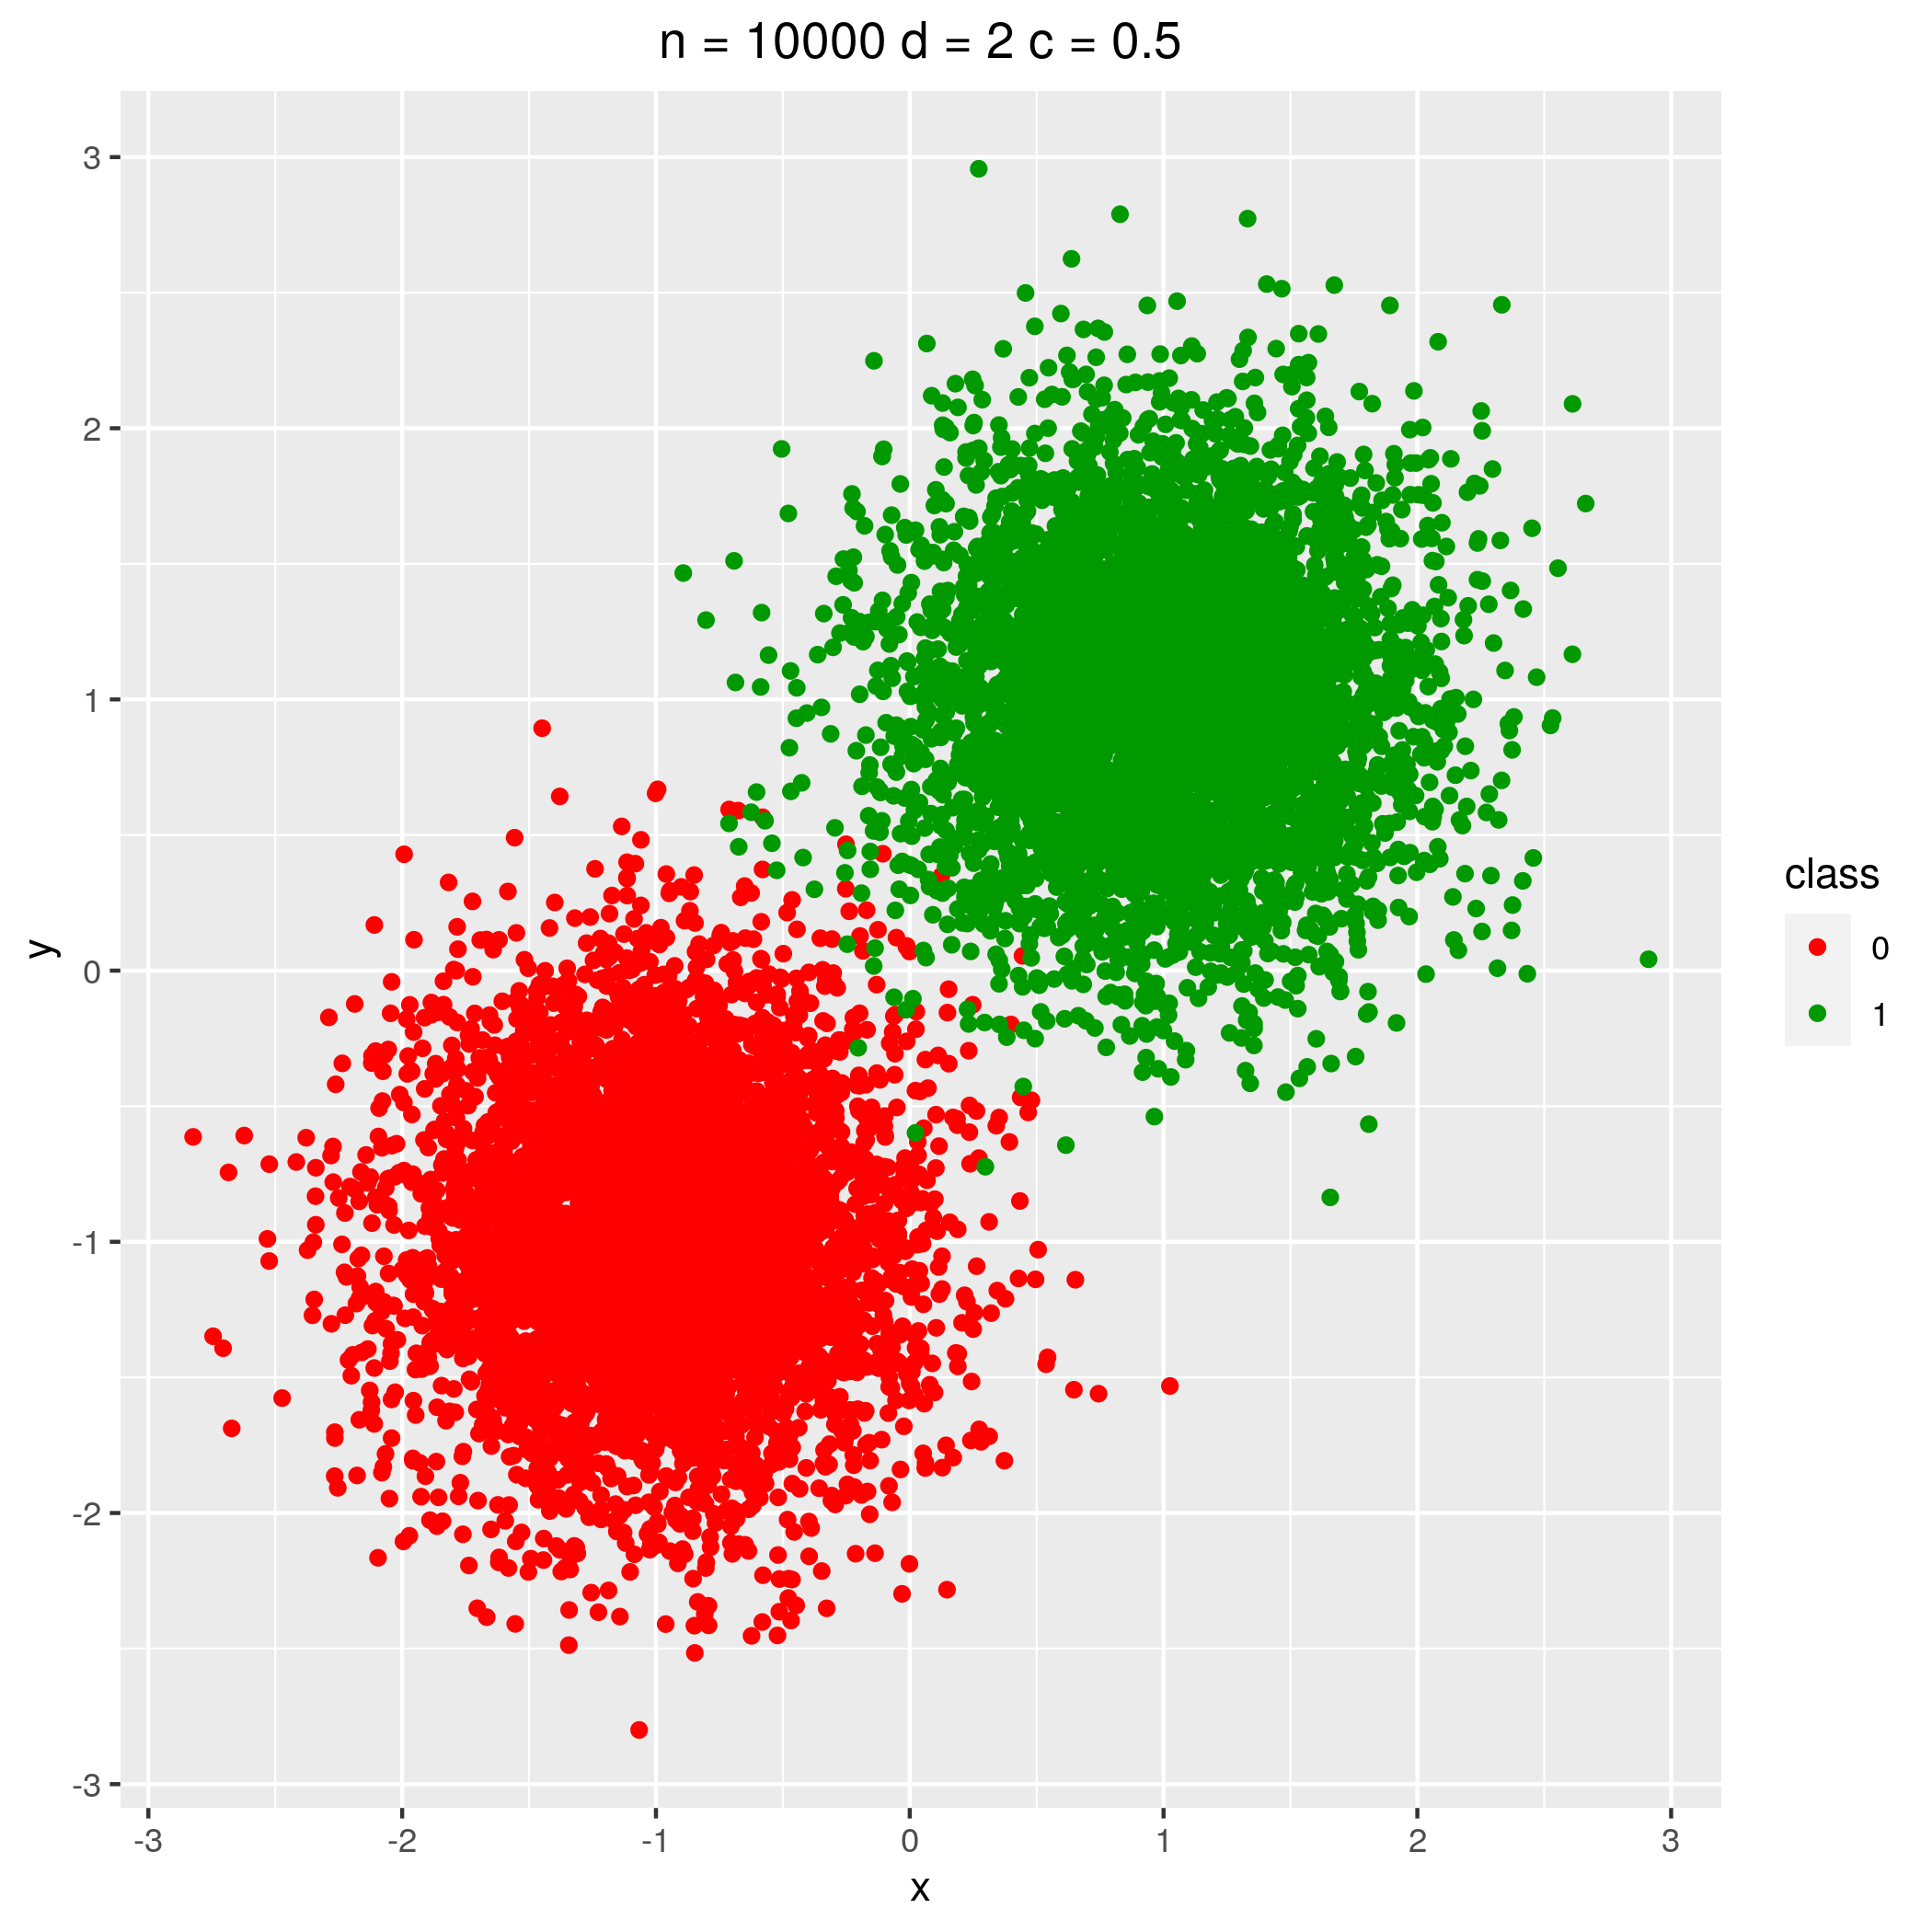
\includegraphics[width=10cm,height=10cm]{diagonal1}

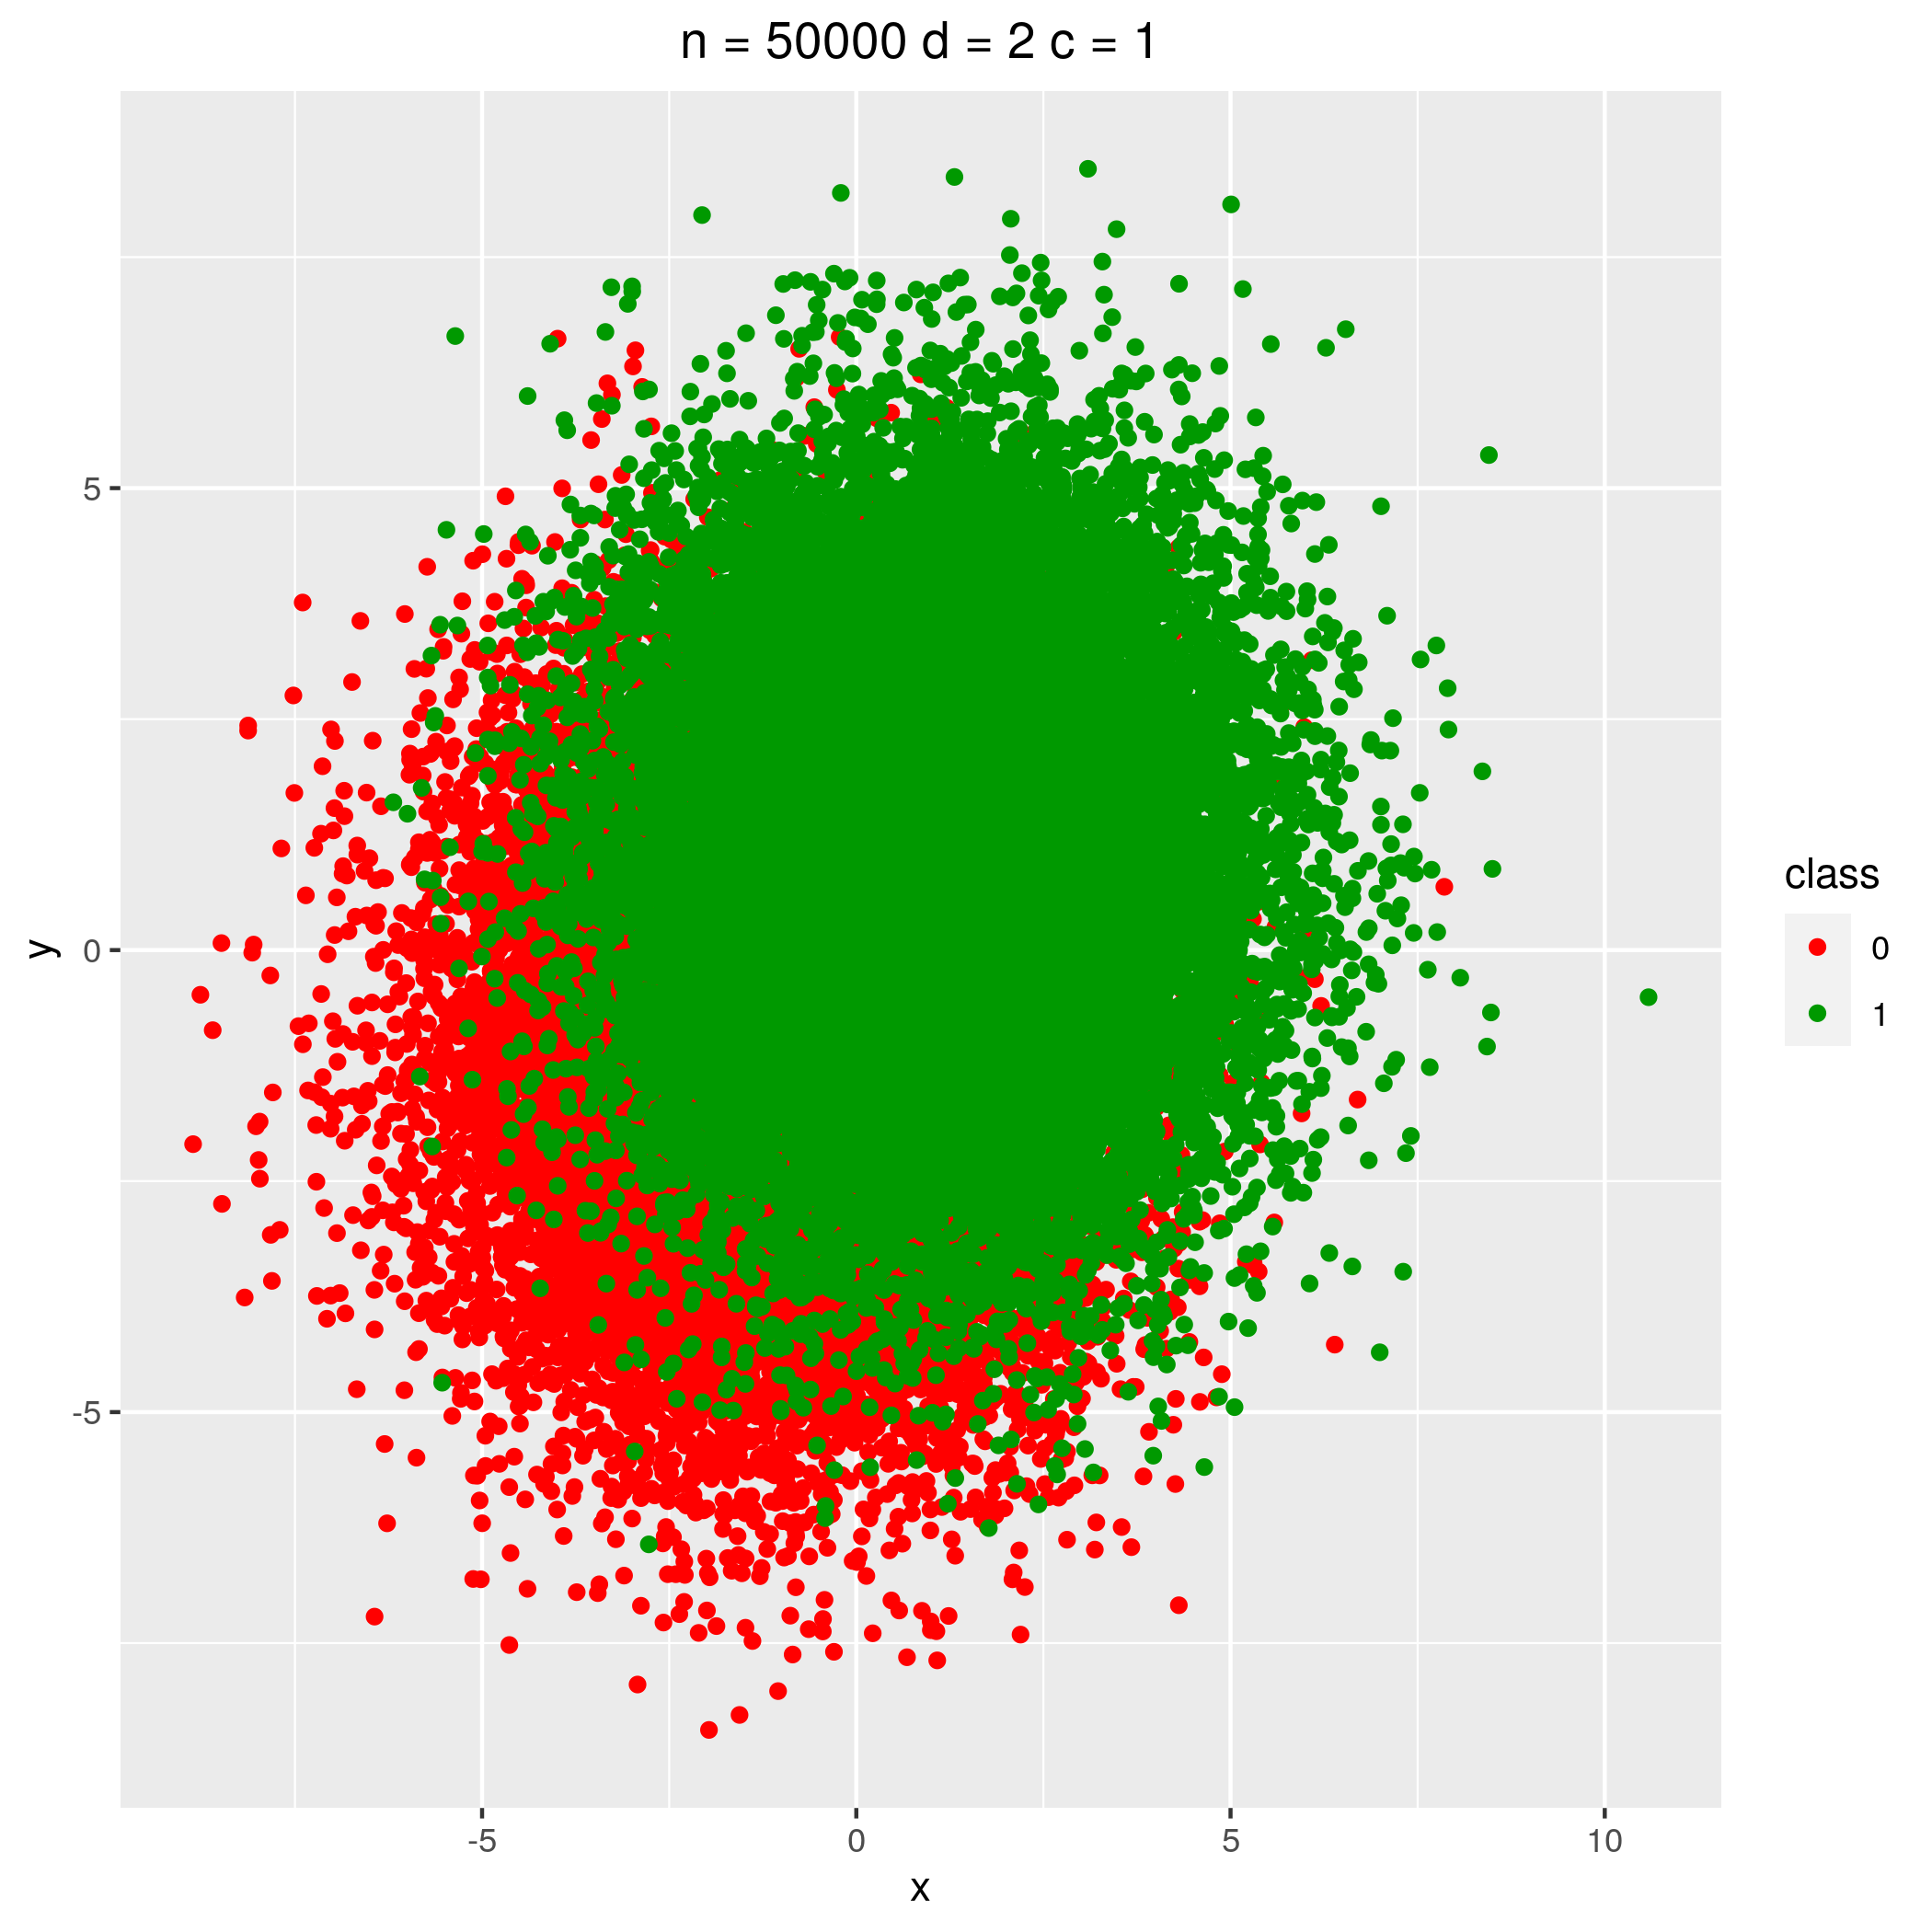
\includegraphics[width=10cm,height=10cm]{diagonal2}

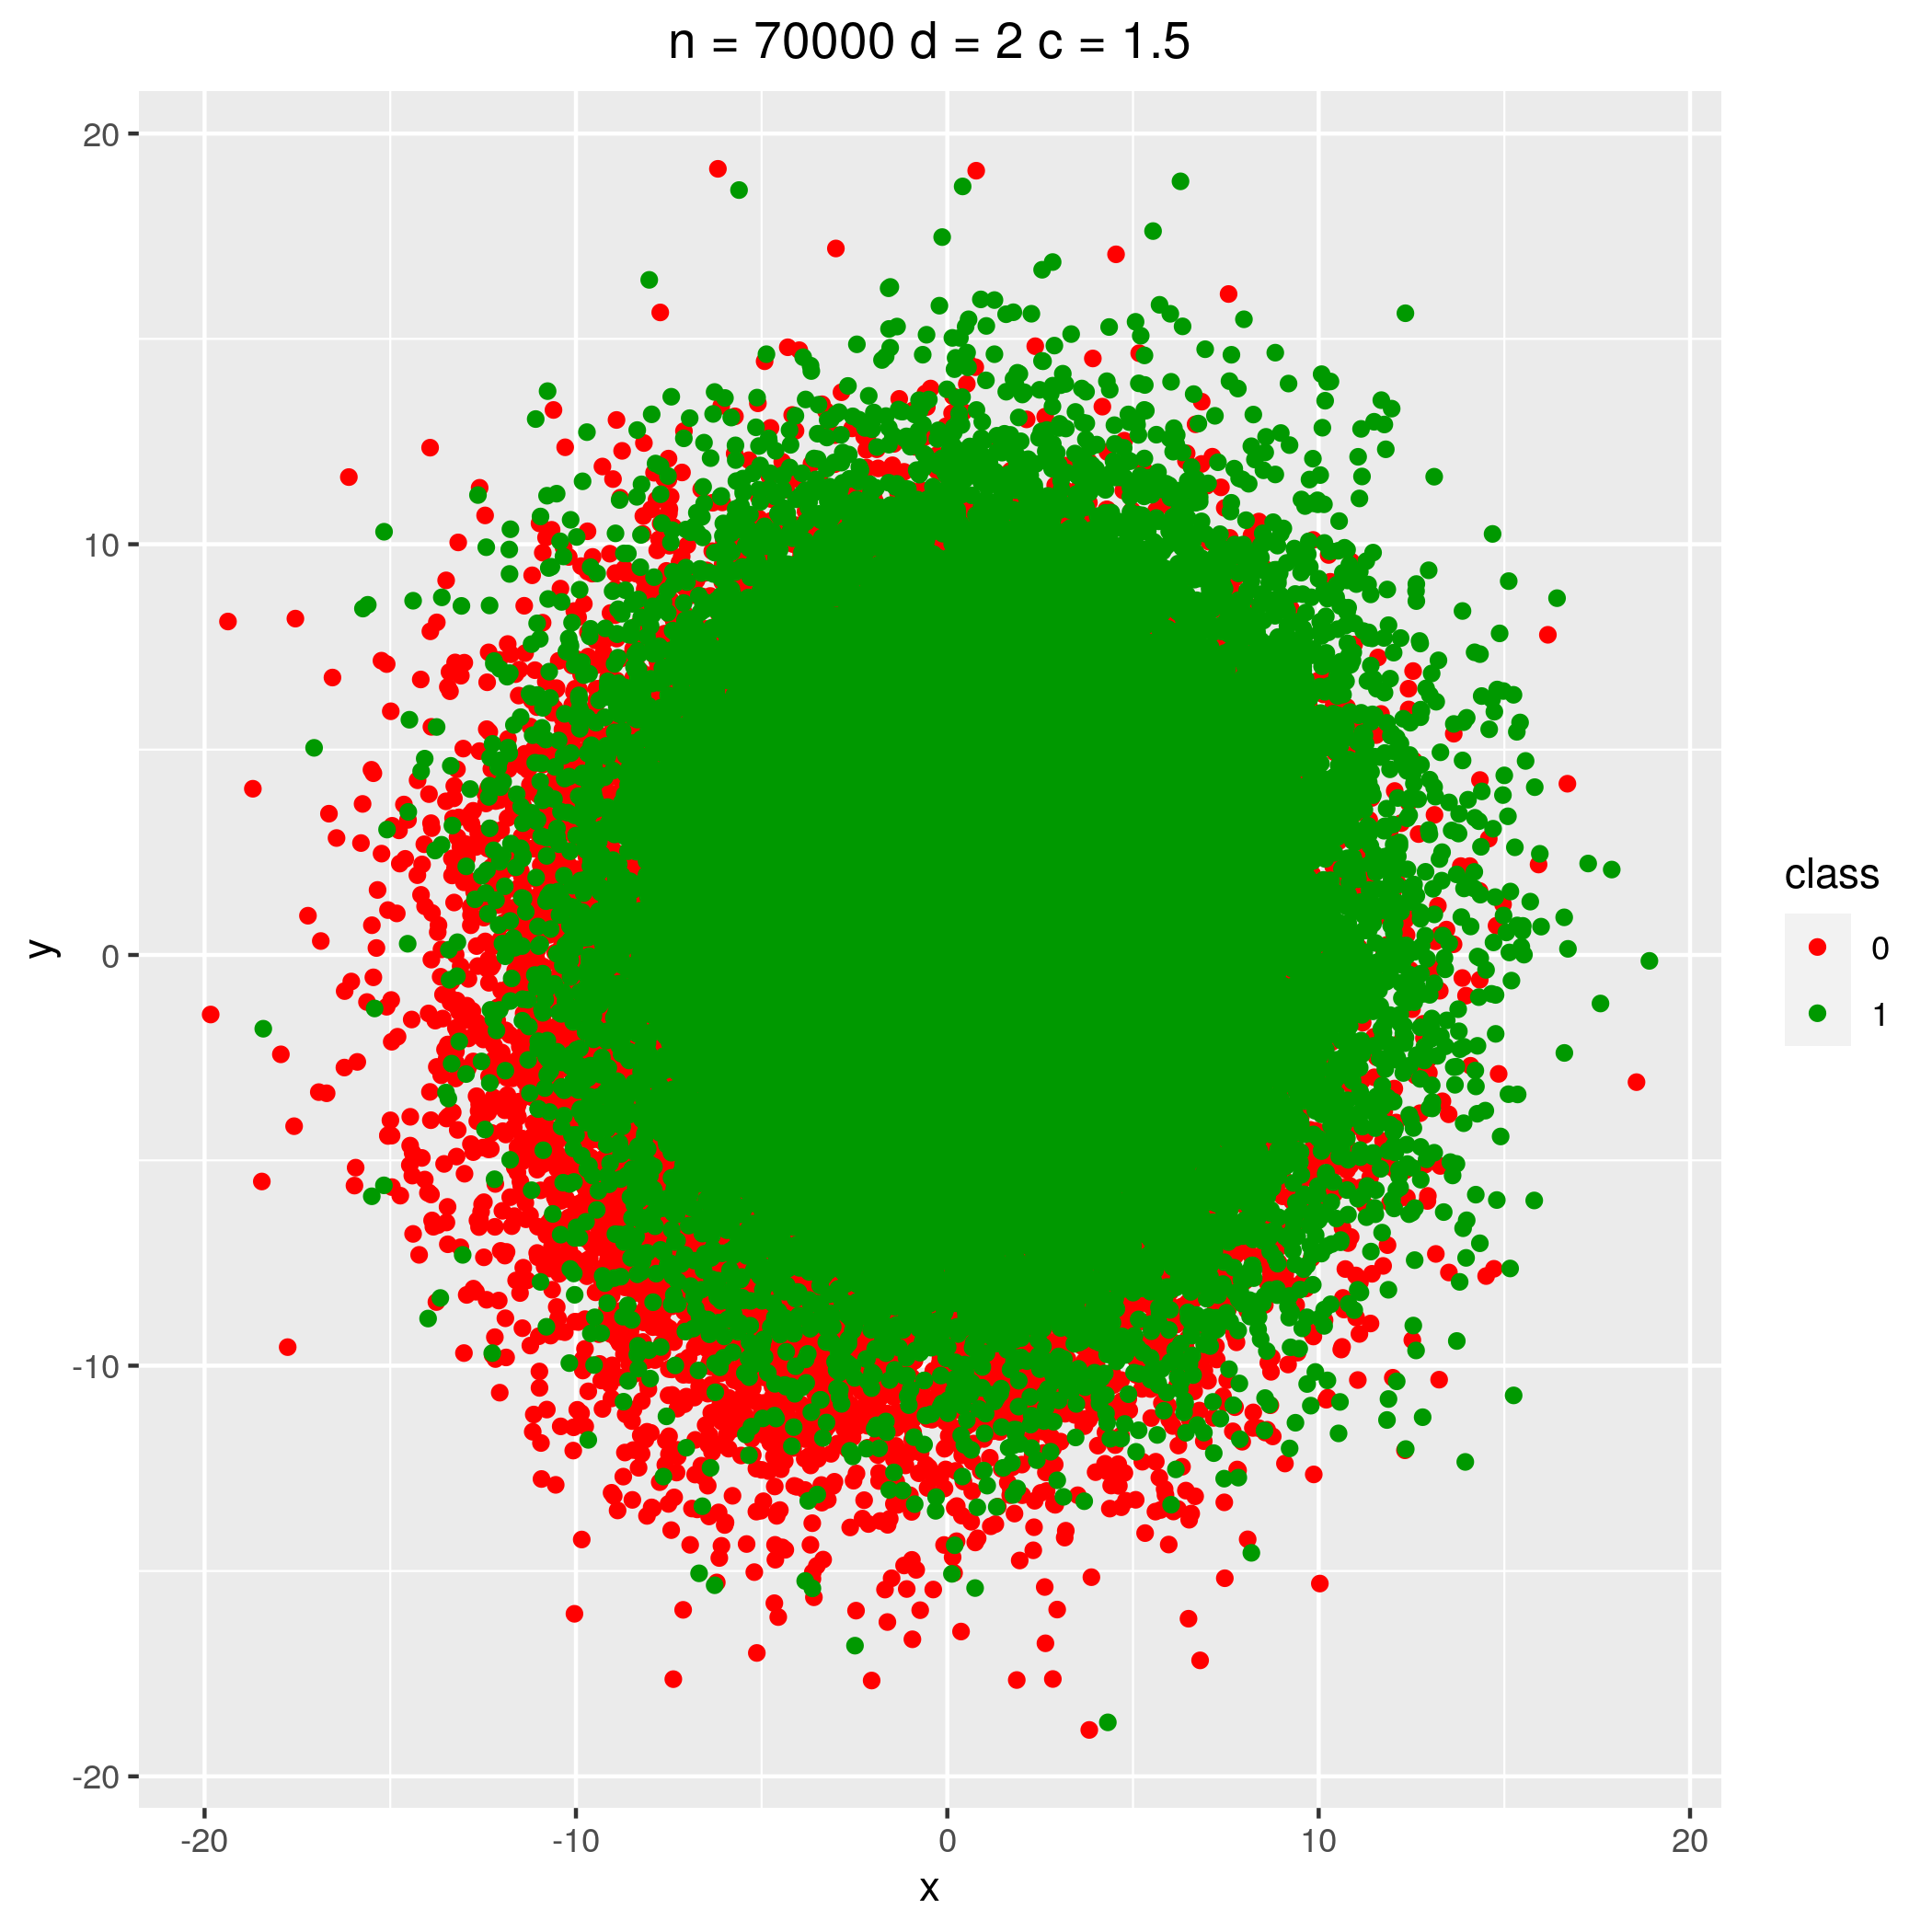
\includegraphics[width=10cm,height=10cm]{diagonal3}

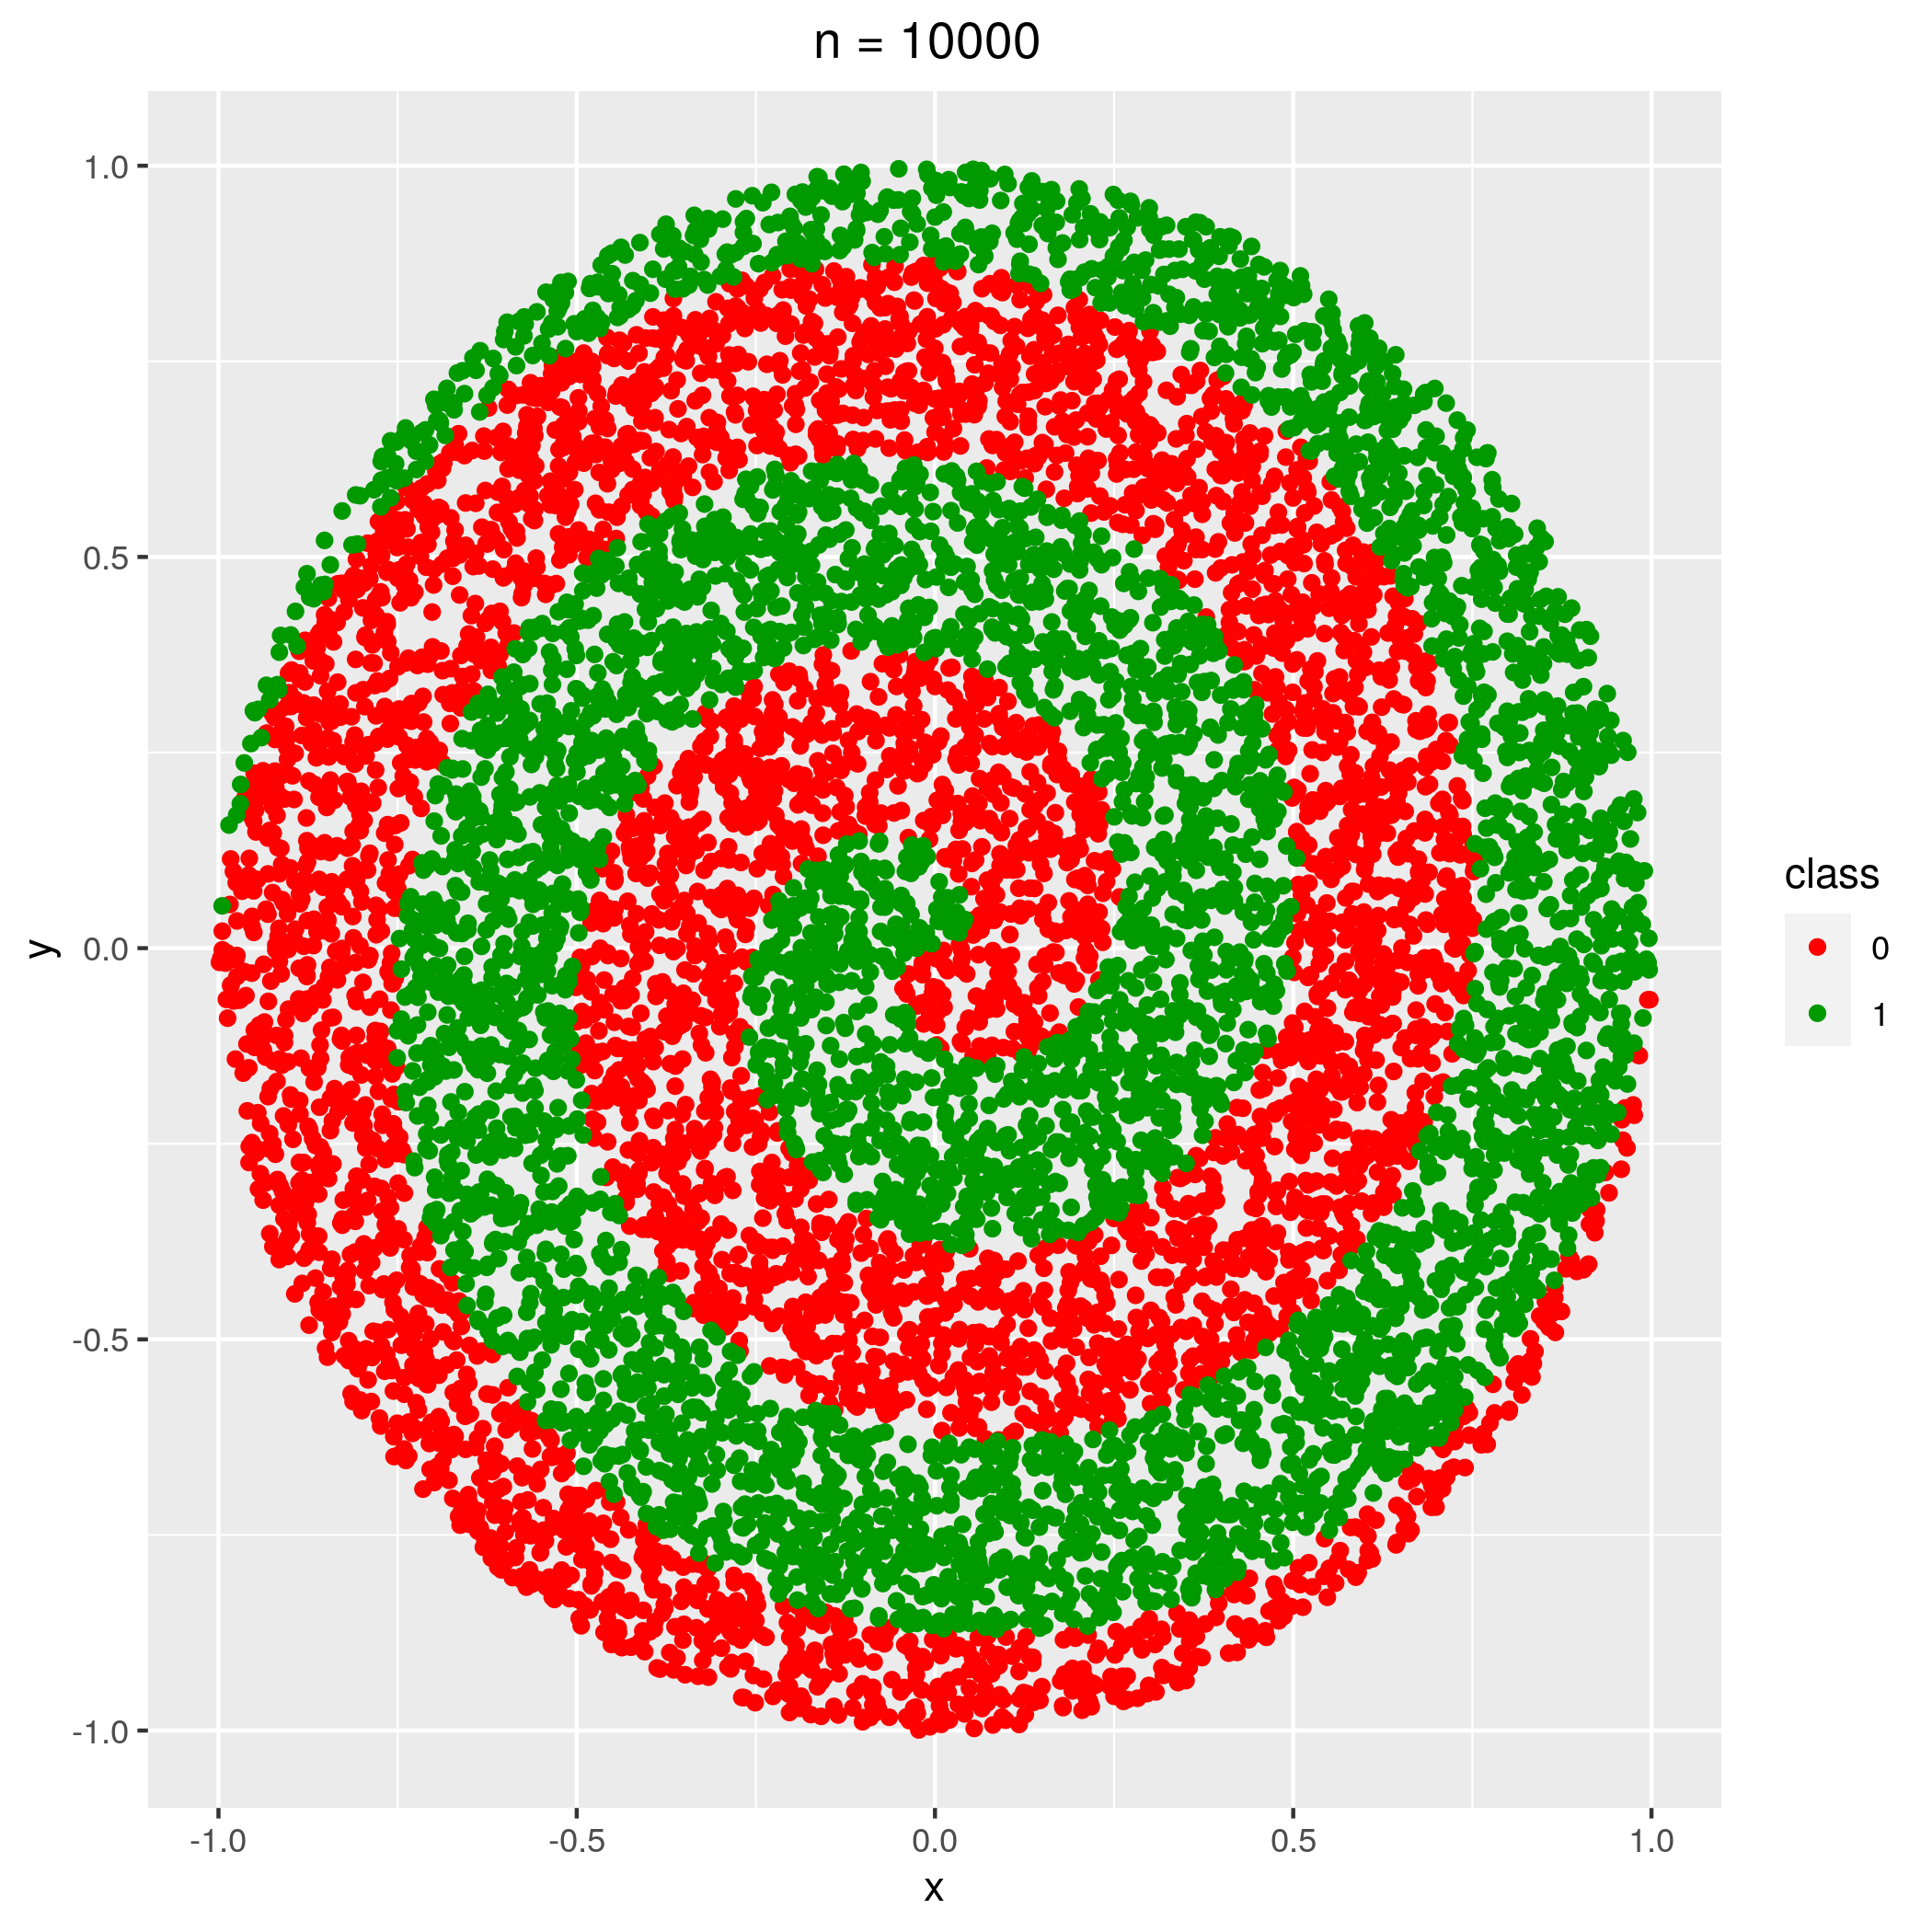
\includegraphics[width=10cm,height=10cm]{espiral1}

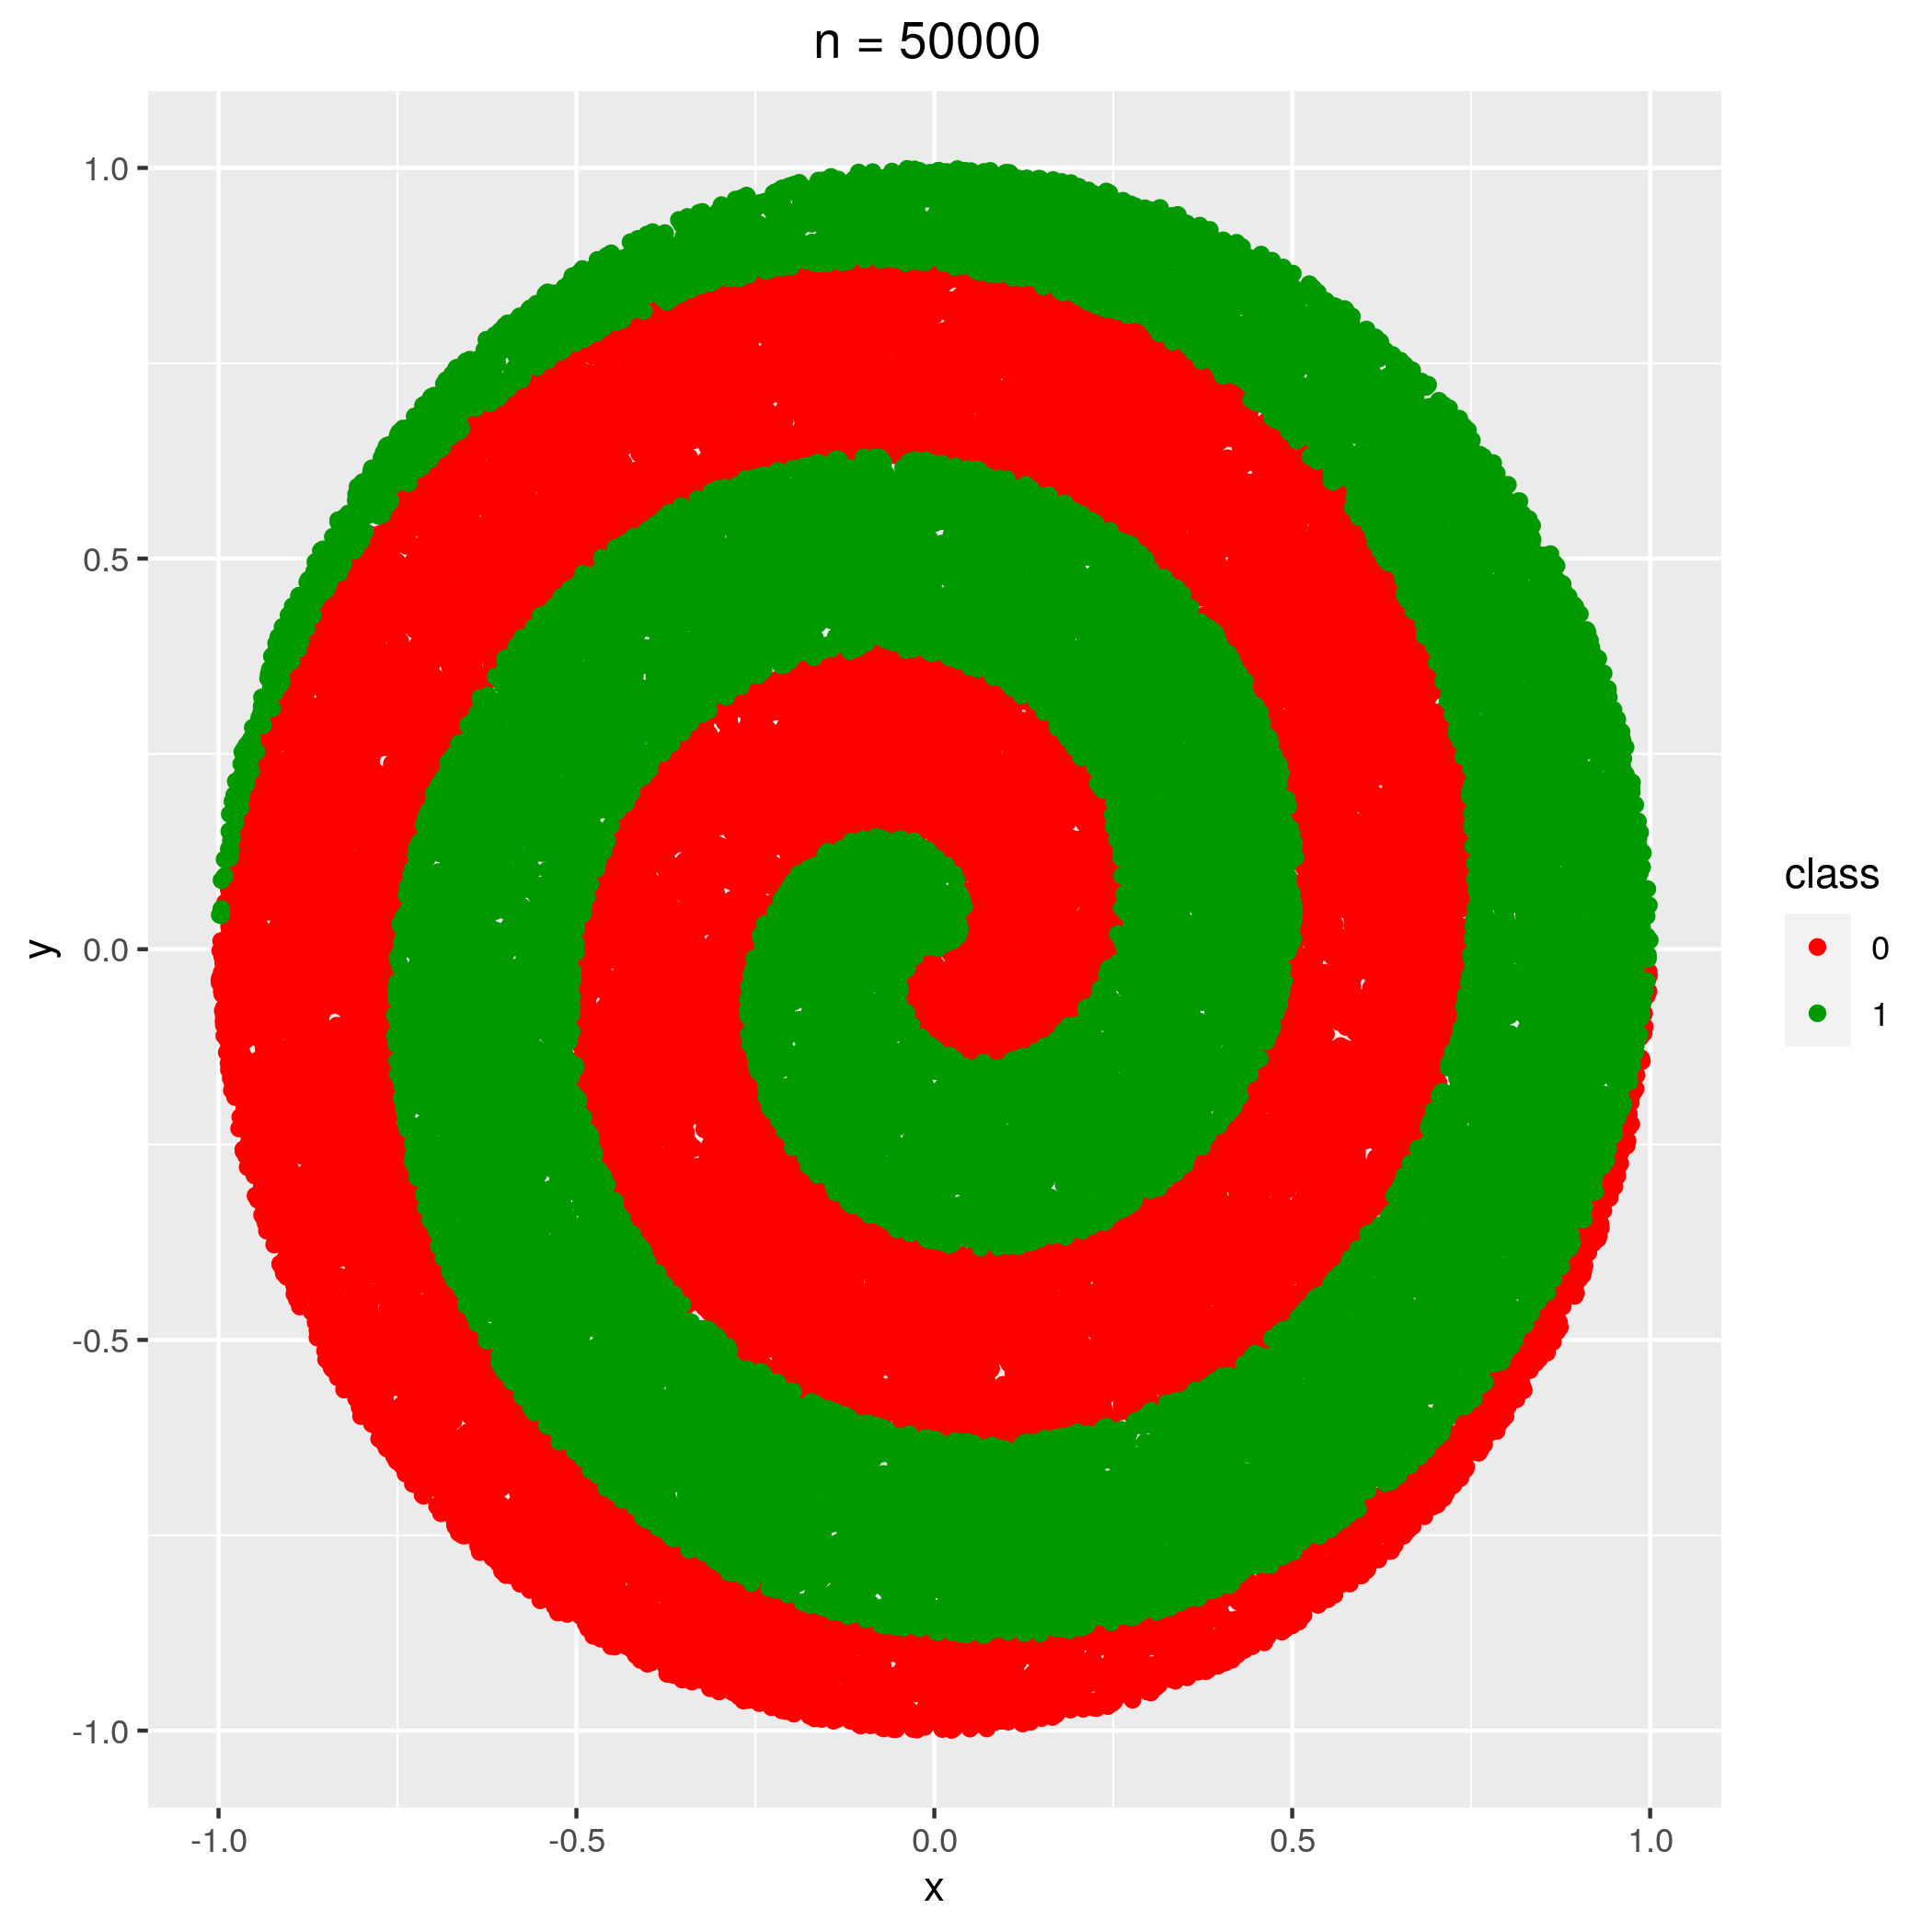
\includegraphics[width=10cm,height=10cm]{espiral2}

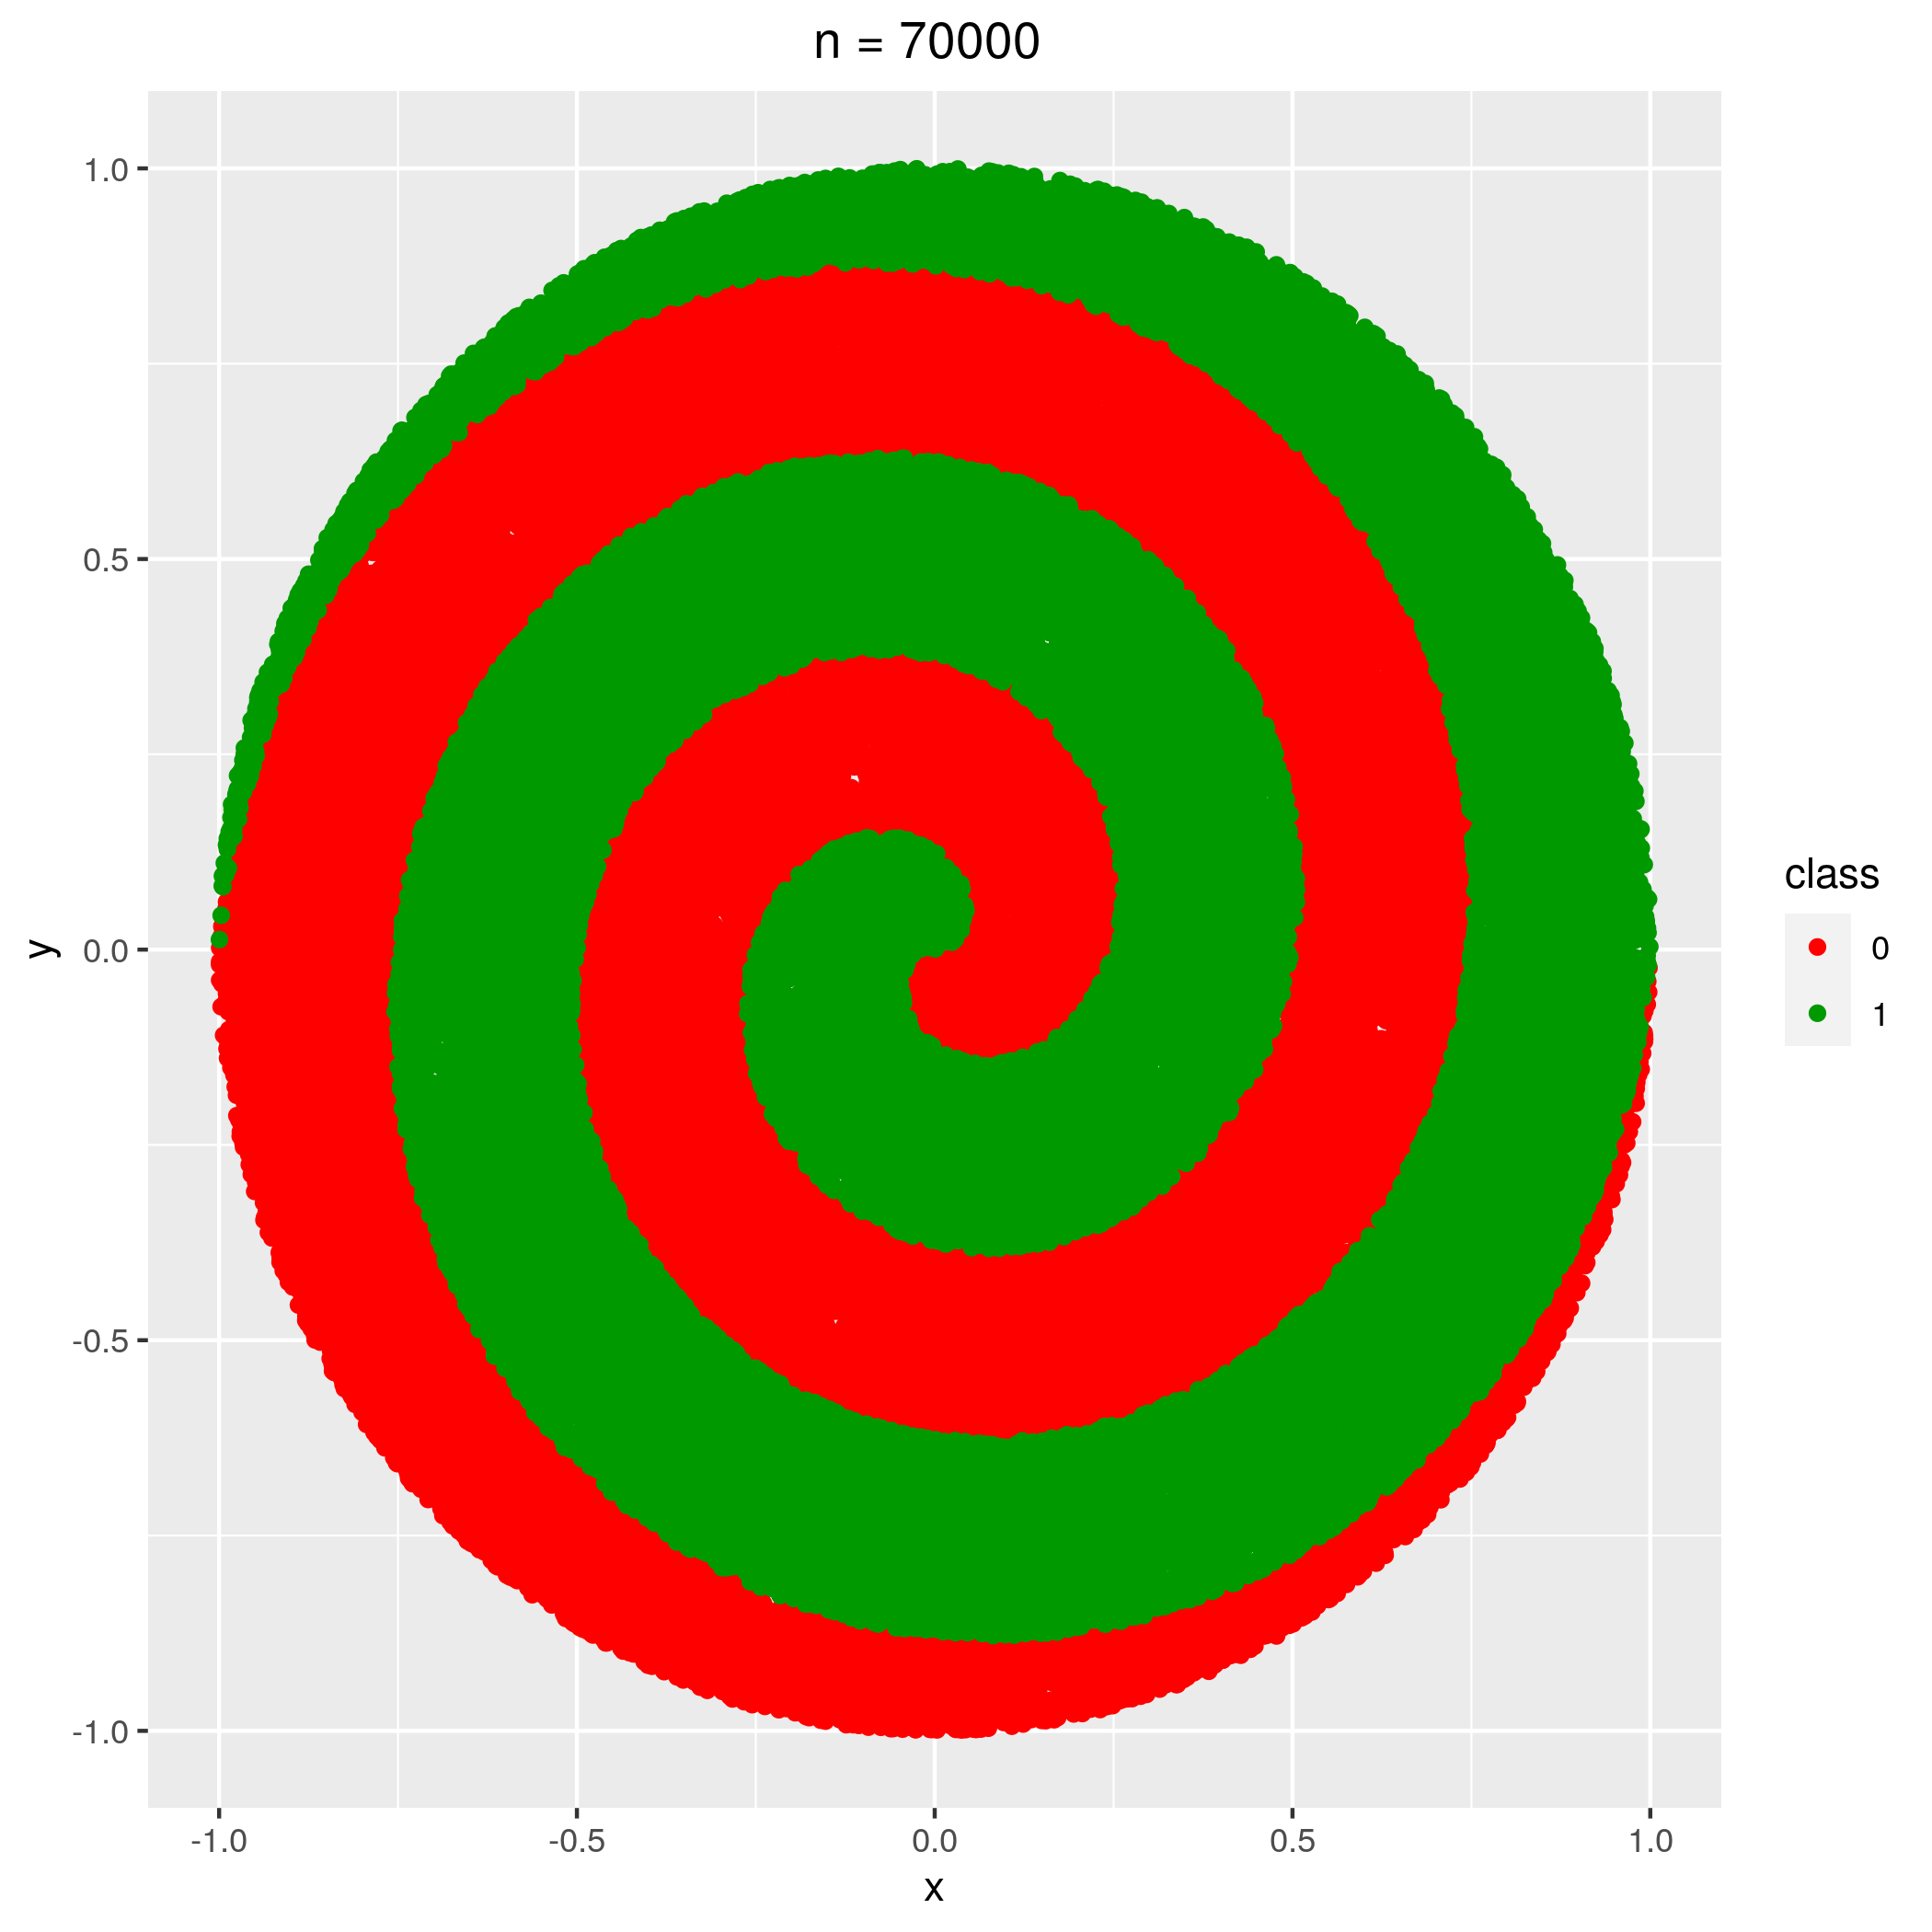
\includegraphics[width=10cm,height=10cm]{espiral3}

\subsection*{3)}

Cross validation usa 4/5 del training set para formar el modelo y
1/5 para testear en cada iteraci�n del 5 fold y ajustar los par�metros
libres de cada problema (el k de KNN y el cp de decision tree), sin
cross validation se usan el training set completo para formar el modelo
y evaluar sobre test para cada valor de par�metro de una amplia gama
que nosotros mismos definimos.

Finalmente se crean modelos usando los par�metros optimizados y se
evalua sobre test, teniendo mejores resultados con par�metros que
fueron optimizados sobre un training set de mayor tama�o, es decir
sin cross validation. 

Por otro lado, el m�todo local (knn) logra mejores resultados que
el m�todo global (decision tree) aunque tambi�n es m�s costoso porque
debe computar todas las distancias euclideas entre el training set
y el punto que se quiere clasificar. 
\end{document}
